\chapter{Marco teórico y estado del arte}

\section{Marco teórico}

El presente capítulo establece los fundamentos conceptuales, metodológicos y tecnológicos que sustentan el diseño e implementación de sistemas automatizados para el análisis del comportamiento estudiantil en entornos digitales. Con el propósito de abordar el fenómeno de estudio bajo una estructura deductiva —partiendo de lo general hacia lo particular—, la revisión de la literatura se organiza en tres ejes temáticos. En primera instancia, se examina el paradigma del modelado de usuarios y su especialización en el ámbito educativo, trazando su evolución desde los esquemas estáticos tradicionales hacia el modelado dinámico e interpretable basado en flujos continuos de información. En segundo lugar, se abordan los métodos analíticos que hacen posible la construcción de dichos perfiles, profundizando en la Minería de Datos Educativos, el agrupamiento incremental sobre flujos de datos y la Minería de Procesos Educativos. Finalmente, se describe el soporte de infraestructura necesario para operar estos modelos, contemplando las fuentes de información institucionales —con énfasis en los Sistemas de Gestión de Aprendizaje (LMS, por sus siglas en inglés)—, el proceso técnico de consolidación de conjuntos de datos y las arquitecturas de software orientadas a eventos.

\subsection{Modelado de estudiantes y de su comportamiento en línea}

En el dominio de la analítica del aprendizaje y los entornos educativos adaptativos, el modelado de estudiantes (\textit{Student Modeling}) se define como el proceso de construir y actualizar una representación computacional explícita de las características de un alumno, tales como su nivel de dominio cognitivo, preferencias de estudio y patrones conductuales de interacción \cite{Brusilovsky2007, Chrysafiadi2013}. El objetivo principal de este perfilado consiste en permitir que plataformas como los Sistemas de Gestión de Aprendizaje (LMS) adapten los recursos y las intervenciones pedagógicas a las necesidades particulares de cada individuo durante su trayecto formativo \cite{Fischer2001, Chrysafiadi2013}.

Históricamente, la recolección de evidencia para conformar estos perfiles estudiantiles ha transitado por mecanismos estáticos de naturaleza explícita e implícita \cite{Brusilovsky2007, Abyaa2019}. Los métodos explícitos requieren la intervención directa del estudiante a través de cuestionarios diagnósticos aplicados al inicio del curso; no obstante, este esquema presenta sesgos de autopercepción y carece de sensibilidad ante la evolución que experimenta el alumno. Como alternativa, la incorporación de técnicas de Minería de Datos Educativos (EDM) ha permitido inferir perfiles de manera implícita mediante el análisis retrospectivo de los historiales de interacción acumulados \cite{Chrysafiadi2013}. Sin embargo, la literatura advierte que estos modelos operan mayoritariamente bajo un paradigma estático o por lotes (\textit{batch}), asumiendo erróneamente que la conducta del estudiante permanece invariable o evaluándola únicamente cuando el periodo escolar ha concluido \cite{Zahoor2025}.

Dado que el aprendizaje constituye un proceso cognitivo en constante transformación, donde las estrategias de estudio y las rutas de navegación se ajustan frente a la dificultad de los temas, las representaciones estáticas resultan insuficientes para un seguimiento académico oportuno \cite{Abyaa2019, Zahoor2025}. Esta limitación ha impulsado el desarrollo del modelado dinámico de estudiantes (\textit{Dynamic Student Modeling}), el cual concibe al perfil computacional como una estructura viva que se recalibra continuamente conforme ingresan nuevos registros de actividad asíncrona en el LMS. Para sostener esta actualización ininterrumpida sin incurrir en un reprocesamiento exhaustivo, este paradigma se apoya en la minería de flujos de datos (\textit{Data Stream Mining}), procesando la información de manera incremental \cite{Gama2010}. En esta línea, Zavaleta-Sánchez et al. \cite{YeseniaZavaleta-Sanchez2025} proponen un marco metodológico que articula la minería de flujos de datos con el descubrimiento de procesos educativos para modelar la evolución temporal del alumno; en la presente investigación, dicha estructura teórica constituye el núcleo metodológico que se busca automatizar a nivel de ingeniería de software.

Adicionalmente, para que el perfilado dinámico sea adoptado de manera efectiva por la comunidad docente, resulta imperativo evitar sistemas opacos. En el ámbito del aprendizaje automático, la interpretabilidad se define como la capacidad de explicar el funcionamiento interno de un modelo computacional en términos comprensibles para el ser humano \cite{BarredoArrieta2020}. Aplicado al entorno educativo, Lee et al. \cite{Lee2025} sostienen que los sistemas analíticos deben priorizar la transparencia algorítmica. Dentro del presente proyecto, la interpretabilidad constituye un requisito transversal para generar perfiles estudiantiles legibles, cuyas trayectorias de interacción evidencien claramente el porqué de cada actualización o agrupamiento, dotando a los educadores de evidencia empírica rastreable para fundamentar el diseño de intervenciones pedagógicas oportunas.

\subsection{Minería de Datos Educativos y Métodos de Generación de Modelos}

En el contexto de los entornos educativos digitales, la extracción algorítmica de valor a partir de los volúmenes masivos de datos asíncronos generados recae en la Minería de Datos Educativos (\textit{Educational Data Mining}, EDM) \cite{Romero2020}. Esta disciplina proporciona la estructura metodológica para descubrir patrones sistemáticos de interacción y evaluar el desempeño de los estudiantes mediante técnicas computacionales. Investigaciones recientes, como las de Mercado et al. \cite{Mercado2024}, demuestran empíricamente que la aplicación de métodos predictivos de EDM sobre los historiales de navegación permite identificar patrones conductuales tempranos que correlacionan de manera directa con el rendimiento final del alumno.

Para materializar este descubrimiento de patrones y construir computacionalmente los perfiles estudiantiles, la literatura distingue dos métodos fundamentales para la recuperación de datos: el enfoque explícito (manual) y el modelado implícito. El modelado explícito requiere la intervención directa del estudiante o del docente para recopilar información, típicamente a través de cuestionarios o evaluaciones diagnósticas previas. Si bien este mecanismo establece una línea base, resulta estático y propenso a sesgos de autopercepción, ya que no logra capturar la evolución continua del estudiante frente a la dificultad del curso ni refleja su comportamiento empírico real dentro de la plataforma. 

En contraste, el modelado implícito automatiza la recuperación de datos extrayendo conocimiento de manera directa desde los registros de eventos (\textit{logs}) del LMS \cite{Supriyanto2025}. Este enfoque permite que disciplinas complementarias, como la Minería de Procesos Educativos (EPM), auditen y mapeen visualmente las secuencias y rutas de aprendizaje reales en entornos asíncronos \cite{AlQaheri2022}. No obstante, la evidencia advierte que una gran proporción de los esfuerzos de modelado implícito actuales persisten en operar bajo un paradigma de análisis estático o por lotes (\textit{batch}) \cite{Setiadi2025}. En consecuencia, construyen perfiles retrospectivos que no se adaptan ni actualizan incrementalmente conforme el comportamiento del alumno evoluciona durante el ciclo formativo. 

Para superar las limitaciones retrospectivas del modelado implícito tradicional, resulta imperativa la transición hacia un modelado dinámico impulsado por la minería de flujos de datos (\textit{Data Stream Mining}) y el procesamiento basado en eventos (\textit{event-driven}) \cite{Zavaleta-Sanchez2025, Kundavaram2025}. Esta ingesta continua permite que técnicas de aprendizaje no supervisado, como el agrupamiento (\textit{clustering}) evolutivo, ajusten sus distribuciones incrementales en tiempo real \cite{Batool2021}. Finalmente, para que esta automatización implícita posea utilidad práctica, debe regirse bajo el principio de interpretabilidad algorítmica \cite{Lee2025}. Evitando los sistemas opacos o de "caja negra" \cite{Arrieta2020}, el modelado dinámico debe proporcionar una justificación estructural clara, dotando a los educadores de evidencia empírica y rastreable para fundamentar el diseño de intervenciones pedagógicas oportunas \cite{Desai2025}. 

\subsection{Infraestructura de datos y entornos virtuales de aprendizaje}

La operación continua de los métodos analíticos descritos requiere de una infraestructura tecnológica capaz de proveer flujos de datos íntegros y estructurados. En el ecosistema digital de las instituciones educativas coexisten múltiples fuentes de información, entre las que figuran los Sistemas de Información Estudiantil (\textit{Student Information Systems}, SIS) orientados a la gestión de matrículas, historiales académicos y trámites administrativos, los repositorios digitales y los sistemas de gestión bibliotecaria \cite{Turnbull2020}. Sin embargo, mientras que los sistemas administrativos almacenan datos demográficos o calificaciones sumativas de baja frecuencia de actualización, el estudio del comportamiento de aprendizaje demanda fuentes que capturen la actividad cotidiana del alumno. Por esta razón, la fuente de datos primordial para este proyecto son los Sistemas de Gestión de Aprendizaje (LMS).

Un LMS se define como una plataforma de software basada en tecnologías web diseñada para planificar, distribuir, evaluar y gestionar procesos de enseñanza-aprendizaje, registrando de manera sistemática las interacciones entre estudiantes, docentes y recursos didácticos \cite{Turnbull2020}. En el mercado e industria del software educativo existen diversas alternativas de LMS cuyas arquitecturas determinan el grado de detalle y accesibilidad de las bitácoras generadas. En la Tabla~\ref{tab:comparativa_lms} se presenta una comparativa técnica de los principales LMS empleados en el ámbito académico.

\begin{table}[htbp]
\centering
\caption{Comparativa de los principales Sistemas de Gestión de Aprendizaje (LMS) como fuentes de datos educativos.}
\label{tab:comparativa_lms}
\footnotesize
\setlength{\tabcolsep}{4pt}
\renewcommand{\arraystretch}{1.3}
\begin{tabular}{p{0.13\textwidth} p{0.16\textwidth} p{0.20\textwidth} p{0.23\textwidth} p{0.22\textwidth}}
\hline
\textbf{Plataforma LMS} & \textbf{Esquema de licencia} & \textbf{Enfoque principal} & \textbf{Registro de interacciones (\textit{Logs})} & \textbf{Facilidad de extracción analítica} \\ \hline
\textbf{Moodle} & Código abierto (GPL) & Educación superior y diseño constructivista modular & Bitácoras relacionales detalladas a nivel de evento, componente, acción y marca temporal & Alta (acceso directo a base de datos, servicios web y exportación nativa) \\
\textbf{Canvas} & Código abierto (AGPLv3) / Comercial en la nube & Educación superior e interoperabilidad en la nube & Eventos de navegación y actividad capturados mediante servicios de telemetría (\textit{Canvas Data}) & Media-Alta (requiere consumo de APIs REST o exportación de flujos de datos) \\
\textbf{Blackboard Learn} & Propietario / Comercial & Gestión académica institucional a gran escala & Registros de auditoría de sesiones, entregas y acceso a contenidos & Media (acceso restringido por arquitectura propietaria; depende de APIs institucionales) \\
\textbf{Open edX} & Código abierto (AGPL) & Cursos masivos abiertos en línea (MOOC) y aprendizaje a ritmo propio & Eventos de seguimiento en formato JSON generados por interacciones en video y evaluaciones & Alta (orientado a eventos, aunque requiere infraestructura compleja de despliegue) \\
\textbf{Google Classroom} & Propietario (Freemium) & Educación básica, media y gestión ágil de tareas & Registros básicos de entrega de asignaciones y publicaciones en el tablón & Baja (trazas de navegación limitadas; extracción sujeta a APIs de Google Workspace) \\
\textbf{Chamilo} & Código abierto (GPLv3) & Educación presencial apoyada en TIC y capacitación & Reportes de seguimiento de lecciones, tiempos de conexión y evaluaciones & Media-Alta (acceso a base de datos relacional con menor granularidad de eventos que Moodle) \\ \hline
\end{tabular}
\end{table}

Como se aprecia en la Tabla~\ref{tab:comparativa_lms}, entornos de código abierto como Moodle sobresalen en proyectos de minería educativa debido a la transparencia de su esquema relacional y a la riqueza de sus tablas de bitácoras, donde cada clic queda asociado a un usuario, un módulo pedagógico y un instante preciso \cite{Romero2020, Supriyanto2025}. Pese a ello, los datos crudos generados por cualquier LMS presentan un nivel de granularidad excesivamente bajo, además de registros administrativos irrelevantes o eventos redundantes que impiden su consumo directo por parte de los algoritmos de aprendizaje automático \cite{Bogarin2018}.

Para resolver esta brecha técnica resulta indispensable la consolidación del conjunto de datos (\textit{Dataset Consolidation}), proceso que comprende la extracción, limpieza, integración, transformación de formato y abstracción semántica de las trazas crudas para estructurarlas en matrices de características y registros de eventos coherentes \cite{Romero2020, Bogarin2018}. Dentro de este flujo de preprocesamiento, además de filtrar el ruido y estandarizar las marcas de tiempo, resulta fundamental reducir la variabilidad de acciones técnicas agrupándolas en categorías pedagógicas significativas denominadas Eventos de Alto Nivel (\textit{High-Level Events}) en el marco de Zavaleta-Sánchez et al. \cite{YeseniaZavaleta-Sanchez2025}, lo que permite condensar las interacciones por estudiante y ventana temporal antes de su ingreso a los módulos de minería.

Finalmente, para que la recolección y consolidación de estos datos deje de ser una tarea artesanal dependiente de exportaciones manuales, la infraestructura debe sustentarse en el procesamiento de datos basado en eventos (\textit{event-driven}). Este paradigma de ingeniería de software e ingeniería de datos se centra en la captura, transformación y despacho asíncrono de registros en el momento en que se produce un cambio de estado o una acción en la plataforma origen. De acuerdo con Kundavaram \cite{Kundavaram2025}, la implementación de tuberías de datos (\textit{data pipelines}) orientadas a eventos permite automatizar la ingesta y el preprocesamiento de flujos continuos con baja latencia y alta tolerancia a fallos. En el contexto de esta investigación, dicha infraestructura representa el eslabón técnico encargado de acoplar el LMS con los algoritmos de minería de flujos y de procesos, habilitando la actualización automática de los modelos estudiantiles.

\section{Estado del arte}
Para fundamentar la necesidad y viabilidad de este proyecto, se realizó una revisión de la literatura en bases de datos de alto impacto, como IEEE Xplore, ScienceDirect, SpringerLink y Google Académico. Con el propósito de capturar de manera exhaustiva las intersecciones entre las plataformas educativas, la evolución de los perfiles de usuario y las técnicas analíticas avanzadas, la búsqueda se estructuró mediante la siguiente cadena de consulta ampliada: \texttt{("Learning Management System" OR "LMS" OR "e-learning" OR "educational") AND ("user modeling" OR "student modeling" OR "student behavior" OR "learning analytics") AND ("data stream mining" OR "process mining" OR "educational data mining")}. A partir de los resultados obtenidos, los trabajos relacionados se han clasificado en tres ejes temáticos progresivos para contrastar los problemas abordados, los métodos aplicados y su relación con la automatización del modelado estudiantil.

\subsection{Modelos de predicción en la Minería de Datos Educativos}
Una vertiente predominante en la literatura es el uso de la Minería de Datos Educativos (EDM) para evaluar y predecir el rendimiento académico. Investigaciones como la de Mercado et al. \cite{Mercado2024} abordan la predicción oportuna en cursos de ritmo propio aplicando técnicas predictivas sobre los historiales de navegación, logrando identificar patrones tempranos que correlacionan fuertemente con el desempeño final. De manera convergente, autores como Setiadi et al. \cite{Setiadi2025} subrayan que el ruido inherente a los datos de los LMS exige una rigurosa selección de características para optimizar la precisión algorítmica. 

Aunque estos enfoques ilustran el potencial de la analítica para adaptar los sistemas a las necesidades del estudiante, presentan una limitación tecnológica estructural: operan bajo un paradigma de análisis por lotes (\textit{batch}). Estas propuestas generan predicciones estáticas que evalúan al alumno de manera retrospectiva, sin la capacidad de actualizarse continuamente a medida que el comportamiento y las estrategias de aprendizaje evolucionan a lo largo del curso.

\subsection{Modelado dinámico y procesamiento en tiempo real}
La necesidad de superar la naturaleza estática de los perfiles retrospectivos ha impulsado enfoques técnicos orientados a la alta disponibilidad y el procesamiento de flujos. Kundavaram \cite{Kundavaram2025} aborda la dificultad de procesar volúmenes masivos de información proponiendo una arquitectura de ingeniería de datos basada en eventos (\textit{event-driven}), logrando la ingesta de datos asíncronos en tiempo real. 

Paralelamente, desde la perspectiva algorítmica, Zavaleta-Sánchez et al. \cite{Zavaleta-Sanchez2025} proponen un marco teórico que integra la minería de flujos de datos (\textit{Data Stream Mining}) con la minería de procesos para generar modelos que representen verdaderamente la evolución temporal del estudiante. El agrupamiento evolutivo (\textit{stream clustering}) dentro de este paradigma permite segmentar a los usuarios en tiempo real conforme sus niveles de interacción cambian (véase la Figura \ref{fig:ejemplo_clustering}). Si bien el enfoque de infraestructura de Kundavaram \cite{Kundavaram2025} resuelve la latencia, carece de un enfoque pedagógico; por el contrario, la articulación teórica de Zavaleta-Sánchez et al. \cite{Zavaleta-Sanchez2025} constituye la base metodológica que la presente investigación busca automatizar en una plataforma de software.

\begin{figure}[htbp]
    \centering
    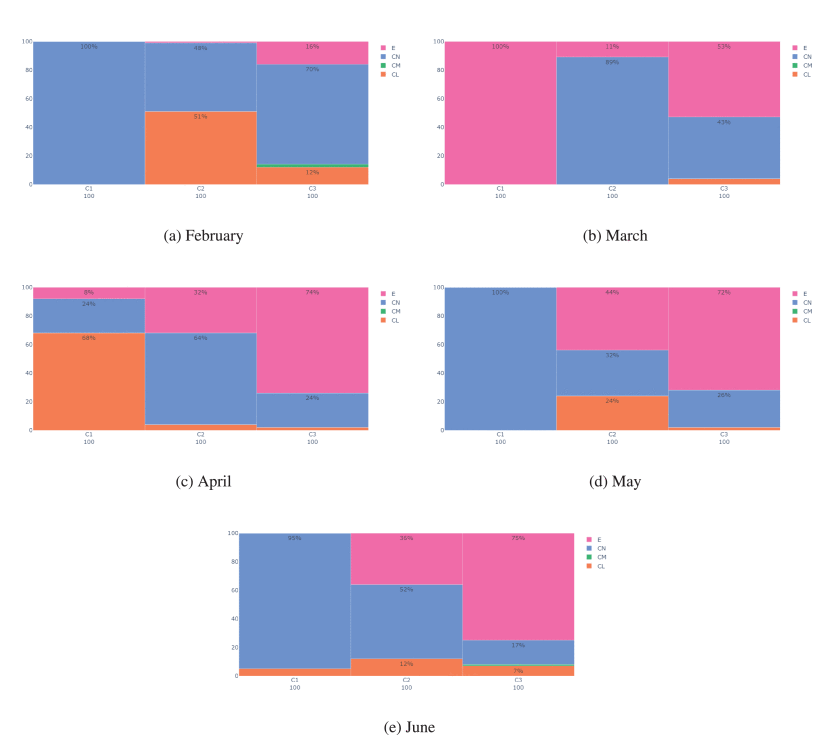
\includegraphics[width=0.8\textwidth]{figuras/ejemplo_clustering.png}
    \caption{Ejemplo de la evolución temporal de perfiles estudiantiles mediante agrupamiento (\textit{clustering}) en flujos de datos. Adaptado de Zavaleta-Sánchez et al. \cite{Zavaleta-Sanchez2025}.}
    \label{fig:ejemplo_clustering}
\end{figure}

\subsection{Minería de procesos educativos e interpretabilidad algorítmica}
Para que las herramientas analíticas dinámicas superen la fase de experimentación y sean adoptadas por la comunidad docente, la precisión computacional debe acompañarse de una estricta transparencia. Investigaciones en Inteligencia Artificial Explicable (XAI) advierten que la opacidad de los modelos predictivos de "caja negra" inhibe su utilidad pedagógica \cite{Lee2025, Desai2025}. Si bien algoritmos tradicionales como los árboles de decisión ofrecen un grado nativo de interpretabilidad mediante reglas lógicas, resultan insuficientes para representar visualmente la naturaleza causal y secuencial del comportamiento humano en un LMS.

Es en este punto donde la Minería de Procesos Educativos (EPM) se integra no solo como técnica de descubrimiento, sino como el motor de explicabilidad del modelo \cite{Supriyanto2025, AlQaheri2022}. Al aplicar técnicas de EPM directamente sobre los subgrupos (clústeres) generados en la fase dinámica, es posible extraer conocimiento empírico sobre cómo interactúa secuencialmente cada perfil. Esto produce grafos de flujo directo (\textit{Directly-Follows Graphs}) que permiten a los educadores visualizar con exactitud qué acciones precedieron a otras, facilitando la comprensión del comportamiento cognitivo del alumno (véase la Figura \ref{fig:ejemplo_grafo}). 

En consecuencia, el método propuesto en esta investigación genera dos salidas analíticas altamente interpretables: 1) el \textbf{modelo del estudiante}, definido por su estado o clúster actual, y 2) el \textbf{grafo de secuencia de interacciones}, que justifica empíricamente dicho estado trazando la ruta de aprendizaje real ejecutada en la plataforma.

\begin{figure}[H]
    \centering
    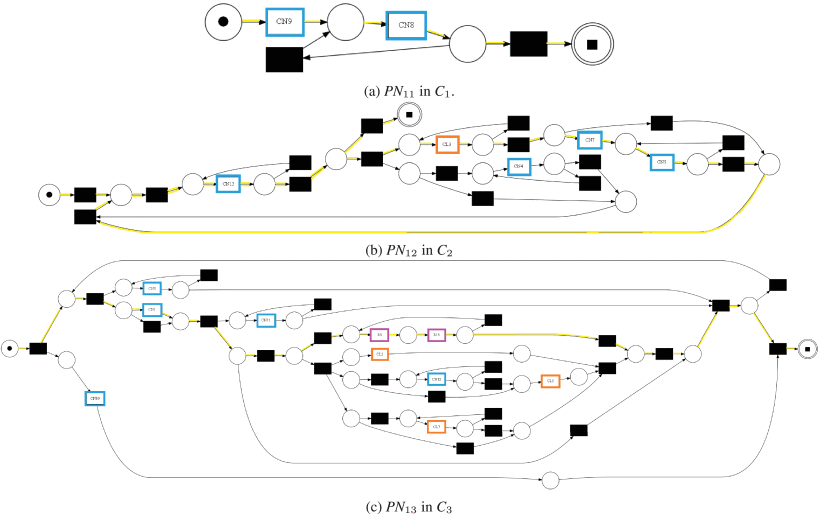
\includegraphics[width=0.85\textwidth]{figuras/ejemplo_grafo.png}
    \caption{Representación interpretable del comportamiento estudiantil mediante un grafo de secuencia de interacciones extraído con EPM. Adaptado de Zavaleta-Sánchez et al. \cite{Zavaleta-Sanchez2025}.}
    \label{fig:ejemplo_grafo}
\end{figure}

\subsection{Conclusión}
A partir de la revisión de la literatura, se evidencia un vacío crítico: la mayoría de los trabajos resuelven problemas aislados, como la predicción estática algorítmica, la gestión pura de infraestructura o el descubrimiento de procesos retrospectivos. A pesar de la existencia de marcos teóricos robustos como el de Zavaleta-Sánchez et al. \cite{Zavaleta-Sanchez2025}, no existe una plataforma de software unificada que automatice este ciclo analítico de extremo a extremo. Este proyecto cubre dicha brecha sistematizando la transición desde la ingesta de eventos hasta la generación de las dos salidas interpretables , garantizando el soporte necesario para la toma de decisiones docentes.